\documentclass[letter,11pt]{article}
%\usepackage[round]{natbib}
\usepackage{setspace} 
\usepackage{dsfont}
\usepackage{amsfonts}
\usepackage{amsmath}
\usepackage{subcaption}
\usepackage{paralist}
%\usepackage{subfig}
\usepackage{times}
\usepackage{latexsym}
\usepackage{graphicx}
\usepackage[T1]{fontenc}
\usepackage{tikz}
\usepackage{url}
\usepackage{pgfplotstable}
\usepackage{titlesec}
\usepackage{color}
\usepackage{lipsum,adjustbox}
\usepackage[font={small}]{caption}
\usetikzlibrary{positioning}

\makeatletter
\newcommand{\@BIBLABEL}{\@emptybiblabel}
\newcommand{\@emptybiblabel}[1]{}
%\makeatother
\usepackage[hidelinks]{hyperref}


\usepackage{acl2012}
\graphicspath{{./plots/}}
\newcommand{\com}[1]{}
\newcommand{\oa}[1]{\footnote{\color{red}OA: #1}}
\newcommand{\lc}[1]{\footnote{\color{green}LC: #1}}

\begin{document}
	
\title{Improved Methodology for Reference-based Evaluation in \\
  Grammatical Error Correction}

%\author{
%  Leshem Choshen\textsuperscript{1} and Omri Abend\textsuperscript{2} \\
%  \textsuperscript{1}School of Computer Science and Engineering,
%  \textsuperscript{2} Department of Cognitive Sciences \\
%  The Hebrew University of Jerusalem \\
%  \texttt{leshem.choshen@mail.huji.ac.il, oabend@cs.huji.ac.il}\\
%}


\maketitle

\begin{abstract}
	
\end{abstract}

\section{Introduction}

% Error correction 
% evaluation in error correction and its centrality
% faithfulness to the source meaning is important, and this has been noted but prev work, and evaluation is geared towards it
% gap in evaluation: however, steps taken to ensure conservativeness in fact push towards formal conservativism by their definition (theoretical claim about the measure)
% this may result in systems that make few changes. indeed we find that this is the case (empirical claim about systems)

% we pursue two approaches to overcome this bias.

% 1. increasing the number of references. this has been proposed before and pursued with m=2, but no assessment of its sufficiency or its added value over m=1 has been made. In order to address this gap we first charachterize the distribution of possible corrections for a sentence. We leverage this characterization to characterize the distribution of the scores as a function of $m$, and consequently assess the biases introduced by taking $m=1,2$ as with previous approaches. 
% We find that taking these values of $m$ drammatically under-estimate the system scores. 
% We back our analysis of these biases with an analysis of the variance of these estimators.
% We analyze the two commonly used scores, the M2 score often used for evalauted, and the accuracy score commonly used in training.

% 2. we note that in fact the important factor is semantic conservativism and explore means to directly assess how semantically conservative systems here through the use of semantic annotation. 
% We use the UCCA scheme as a test case, motivated by HUME.
% First question: is it well-defined on learner language. it is.
% Second question: are corrections in fact semantically conservate? to show that, we need to verify that the corrections make few (if any) semantic changes. our results indicate that this is the case: we show that the corrections are similar in (UCCA) structure to the source.

% conclusion (not in intro): we tried to use semantic similarity to improve systems.
% this is difficult due to semantic conservatism. we expect this will be in issue once evaluation is improved.
% future work.
% also future work: use multiple references in training (did people do that?)

% sections:
% 1. Introduction
% 2. Formal conservativism in GEC
% 3. First approach: Multiple References
% 3.1. A Distribution of Corrections
% 3.2. Scores (M2, accuracy index, accuracy exact)
% 3.3. Data
% 3.4. Bias of the Scores (setup + results)
% 3.5. Variance of the Scores (setup + results)
% 4. Second approach: Semantic Similarity
% 4.1. Semantic Annotation of Learner Language (prev work)
% 4.2. UCCA Scheme (see HUME)
% 4.3. Similarity Measures (including prev work of elior)
% 4.4. Empirical Validation: IAA, semantic conservativism vs. gold std
% 5. Conclusion

Grammatical Error Correction (GEC) is a challenging research field, which interfaces with many
other application areas of linguistics. The field is receiving considerable
interest recently, notably through the GEC-HOO \cite{dale2011helping,dale2012hoo},
CoNLL shared tasks \cite{kao2013conll,ng2014conll}.
Within GEC, considerable effort has been placed on system evaluation,
which is notoriously difficult,
much due to the many valid corrections each source sentence may have
\cite{tetreault2008native,madnani2011they,chodorow2012problems,dahlmeier2012better}.

An important criterion in the evaluation of GEC systems (henceforth, {\it correctors})
is their ability to generate corrections that are faithful to meaning of the source. In fact, many would prefer
a somewhat cumbersome or even an occasionally ungrammatical correction over a correction
that alters the meaning of the source \cite{brockett2006correcting}.
As a result, often when compiling gold standard corrections for the task,
annotators are instructed to be conservative in their corrections, e.g. in NUCLE \footnote{Daniel Dahlmeier, personal communication.} and the Treebank of LL \lc{helen suddenly answered, sent the guidelines and it is very specific in them is it still "personal communication"?}.
A recent attempt to formally capture this precision/recall asymmetry has
been the shift from using $F_1$ to $F_{0.5}$, where Precision is
emphasized over Recall, as a common evaluation measure
in GEC \cite{dahlmeier2012better}.

However, favoring precision over recall may lead to reluctance of correctors to make any changes (henceforth, {\it over-conservatism}).
Using a single reference correction (a common practice in GEC) compounds this problem,
as systems are not only penalized more for making an incorrect change (over not making
any change), but are often penalized for any correct change not found in the reference.

We present results that indicate that current state of the art systems suffers
from over-conservatism. Evaluating the output of 15 state
of the art GEC systems that participated
in the recent CoNLL2014 shared task, we find that all of them
substantially under-predict corrections relative to the gold standard
(\S\ref{sec:formal_conservatism}). 

We pursue two approaches to address this gap, proposing
improved reference-based protocols to decrease penalties of valid correction. Thus, avoiding over-conservatism.
First, we study the effect of increasing the amount of references
(henceforth, $M$) (\S\ref{sec:increase-reference}).
While previous evaluation explored the case of $M=2$,
no empirical assessment has been carried out, of its sufficiency
or its added value over $M=1$.
In our experiments we estimate the number of corrections necessary
to cover the bulk of the distribution of possible corrections.
We then consider two measures for
assessing the validity of a proposed correction relative to a set of references,
and characterize the distribution of their scores as a function of $M$.
We find that assessment based on $M=1$ or $M=2$ dramatically under-estimate
the true performance of the systems (\S\ref{sec:increase-reference}). 
We conclude with an analysis of
the statistical significance of these evaluation protocols.

Second, we pursue an alternative way of determining whether a correction faithfully
represents the semantics of the source, by developing a semantic measure based
on the similarity of their {\it semantic} structures (\S\ref{sec:Semantics}).
We define a measure, using the UCCA scheme \cite{abend2013universal} as a
test case, motivated by its recent use for machine translation
evaluation \cite{birch2016hume}.
In order to assess the feasibility of this approach, we annotate a
section of the NUCLE \cite{dahlmeier2013building}
parallel corpus. Our results support the feasibility of the proposed approach,
by showing that semantic structural annotation can be consistently applied
to LL and that manually compiled references do indeed
have similar semantic structures to those of their source sentences.

The two approaches address the insufficiency of using too few references from
complementary angles. 
The first attempts to cover the bulk of the distribution of possible
corrections for a sentence, while the second
uses semantic instead of string similarity, in order to abstract away
from some of the formal variation between different valid corrections.

\section{Over-Conservativism in GEC Systems}\label{sec:formal_conservatism}

%The field of GEC was always thriving for conservatism in its corrections, with the prominent example of using
%$F_{0.5}$ emphasizing precision over recall(\cite{ng2014conll}). we wish to highlight the problem that
%arises from pursuing this conservatism as done today.
%Then, we wished to be conservative, and we achieved that, why shouldn't we rejoice just yet? Theoretically, we might be progressing towards not correcting at all, instead of progressing towards correcting more accurately. 

%Manual analysis showed excessive formal conservatism and under correction.
%Albeit important, manual analysis is not enough and we aimed for generating some quantitative measures. 

In this section we demonstrate that current correctors
suffer from over-conservatism: they tend to make too few changes to the source. 


\paragraph{Experimental Setup:}\label{par:experimental_setup}

Our experiments are on the NUCLE dataset,
a parallel corpus of learner language (LL) paragraphs and their corrected versions,
which is the de facto standard in GEC.
The corpus contains paragraphs in LL, each of about 400 words.

We evaluate all participating systems in the CoNLL 2014,
in addition to the best performing system on this dataset \cite{rozovskaya2014building}.
The particiapting systems and their abbreviations are: Adam Mickiewicz University (AMU),
University of Cambridge (CAMB), Columbia University and the University of Illinois at Urbana-Champaign (CUUI),
Indian Institute of Technology, Bombay (IITB), Instituto Politecnico Nacional (IPN),
National Tsing Hua University (NTHU), Peking University (PKU), Pohang University of Science and Technology (POST),
Research Institute for Artificial Intelligence, Romanian Academy (RAC), Shanghai Jiao Tong University (SJTU),
University of Franche-Comte (UFC), University of Macau (UMC),
Rozovskaya and Roth's best performing system (RoRo) \cite{rozovskaya2016grammatical}.
All are trained and tested on the NUCLE corpus.

We compare the prevalence of changes made by the correctors to the source,
to the one made by a NUCLE reference to the source.
We discarded from our evaluation all non-alphanumeric
characters, both within tokens or as token on their own.

%In order to have better evaluation of the real goal of corrections we also
%compute all of the measures on ,
%based on the Cambridge First Certificate in English
%(FCE) \cite{yannakoudakis2011new},
%a new large parallel corpus containing only ungrammatical sentences of learners
%native of different languages.


\paragraph{Measures of Conservatism:}
We measure the divergence between the source and the reference in three ways.

First, we measure to what extent \emph{words} were changed; altered, deleted or added.
We compute word alignment, and then
count the number of unaligned words and the aligned words that  do not match.
We formulate the alignment problem as a weighted bipartite graph matching problem,
placing the source and corrected tokens on the two sides of the graph.
Edge weights are assigned to be the edit distance between the tokens.
\footnote{When breaking ties, we favor alignments where the place in the sentence is closer.}
We note that aligning words in GEC is much simpler than in machine translation,
as most of the words are kept unchanged, deleted fully, added, or changed slightly.

Second, we quantify word \emph{order} differences 
by computing Spearman's $\rho$ on the alignment considered above.
$\rho$ is lower as more order changes exist.

Third, we align
\emph{sentences} and count how many sentences were split
and how many concatenated.


\begin{figure}[tbp]
  \centering
  \begin{subfigure}[]{0.4\textwidth}
  	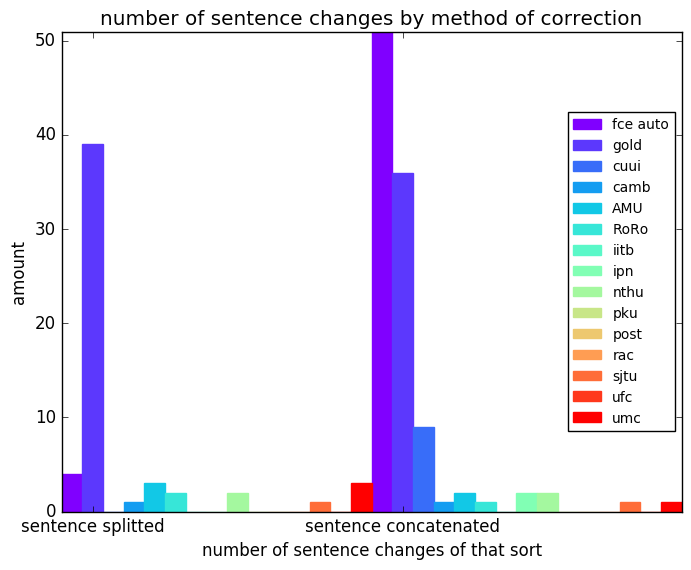
\includegraphics[width = \textwidth]{aligned}
  	\caption{Number of source sentences (y-axis) split 
  		(right bars) or concatenated (left bars) in the correction, according to the gold standard (striped column) and different correctors (colored columns). The gold standard makes about an order of magnitude more splits and concatenations than the correctors.\label{fig:split}}
  \end{subfigure}

  \begin{subfigure}[]{0.4\textwidth}
  	\com{\caption{\label{fig:rho}}}
    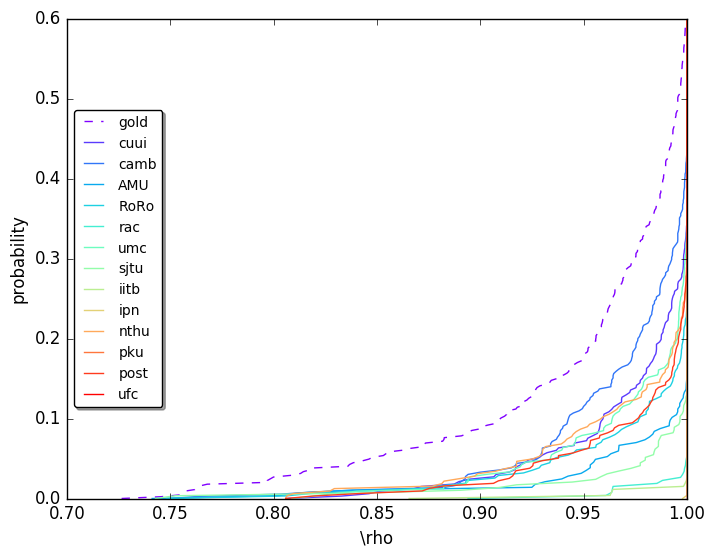
\includegraphics[width = \textwidth]{spearman_ecdf}
    \caption{Empirical cumulative probability (y-axis) of a sentence to get Spearman's rho values (x-axis) of word alignment. The gold standard(dotted line) makes word change alterations to more sentences than the correctors, and within these sentences, it changes order more substantially.\label{fig:rho}}
  \end{subfigure}

  \begin{subfigure}[]{0.4\textwidth}
  	%\caption{\label{fig:words_changed}}
  	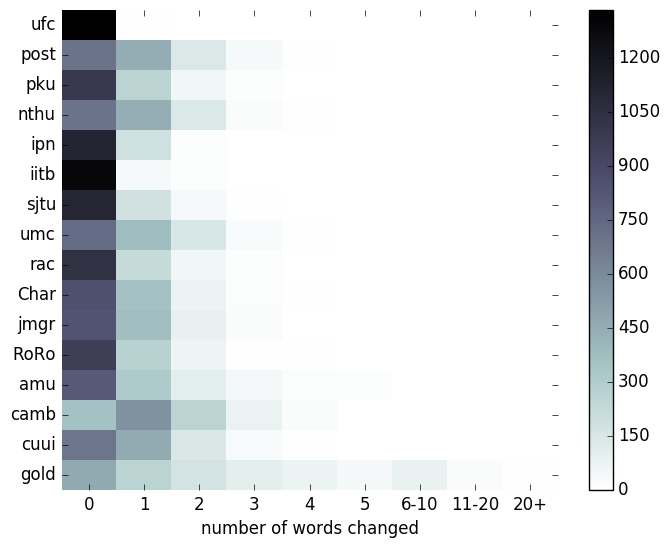
\includegraphics[width = \textwidth]{words_differences_heat}
  	\caption{Amount of sentences(heat) by number of words changed(x-axis) per system(y-label). The gold standard(bottom) corrects more words per sentences and more sentences relative to other systems.\label{fig:words_changed}}
  \end{subfigure}
  \com{\caption{(a) Number of source sentences (y-axis) split 
  		(right bars) or concatenated (left bars) in the correction, according to the gold standard (striped column) and different correctors (colored columns). The gold standard makes about an order of magnitude more splits and concatenations than the correctors.\\
  		(b) Empirical cumulative probability (y-axis) of a sentence to get Spearman's rho values (x-axis) of word alignment. The gold standard(dotted line) makes word change alterations to more sentences than the correctors, and within these sentences, it changes order more substantially.\\
  		(c) Amount of sentences(heat) by number of words changed(x-axis) per system(y-label). The gold standard(bottom) corrects more words per sentences and more sentences relative to other systems.\\
  		See \S\ref{par:experimental_setup} for a legend
  		of the systems.}\label{fig:over-conservatism}}
  \caption{\label{fig:over-conservatism}
    See \S\ref{par:experimental_setup} for a legend
    of the systems.}
  
  \com{
  	\begin{figure}[tbp]
  		\centering
  		\begin{subfigure}[]{0.4\textwidth}
  			\caption{\label{fig:split}}
  			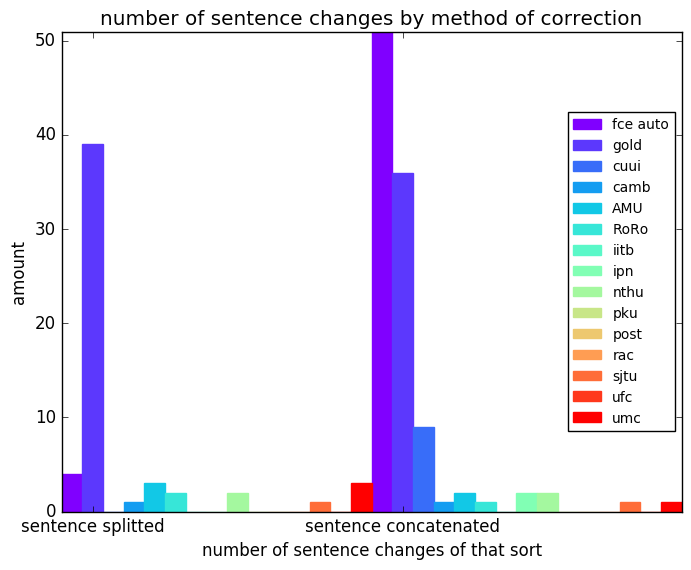
\includegraphics[width = \textwidth]{aligned}
  			\com{\caption{Number of source sentences (y-axis) split 
  					(right bars) or concatenated (left bars) in the correction, according to the gold standard (striped column) and different correctors (colored columns). The gold standard makes about an order of magnitude more splits and concatenations than the correctors.\label{fig:split}}}
  		\end{subfigure}
  		
  		\begin{subfigure}[]{0.4\textwidth}
  			\caption{\label{fig:rho}}
  			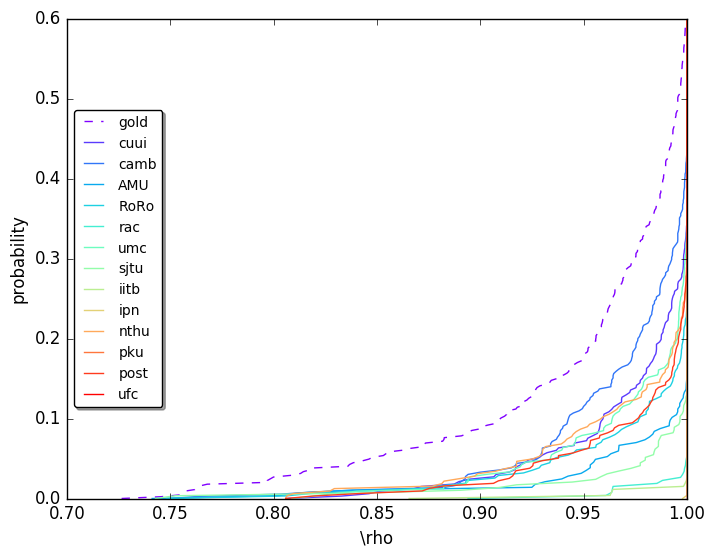
\includegraphics[width = \textwidth]{spearman_ecdf}
  			\com{\caption{Empirical cumulative probability (y-axis) of a sentence to get Spearman's rho values (x-axis) of word alignment. The gold standard(dotted line) makes word change alterations to more sentences than the correctors, and within these sentences, it changes order more substantially.\label{fig:rho}}}
  		\end{subfigure}
  		
  		\begin{subfigure}[]{0.4\textwidth}
  			\caption{\label{fig:words_changed}}
  			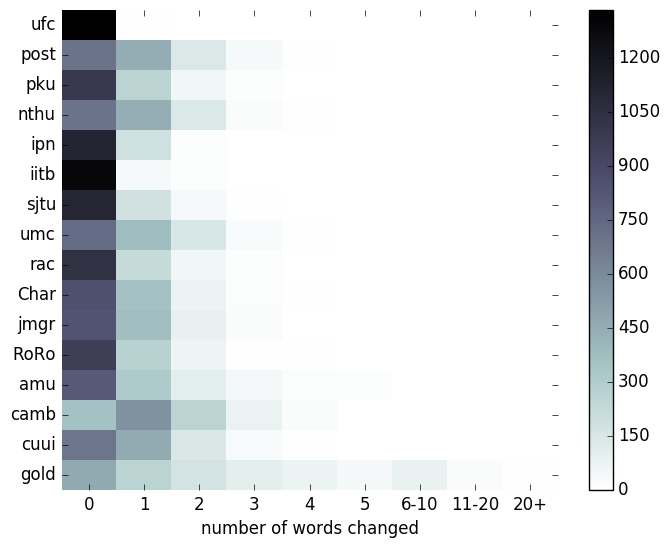
\includegraphics[width = \textwidth]{words_differences_heat}
  			\com{\caption{Amount of sentences(heat) by number of words changed(x-axis) per system(y-label). The gold standard(bottom) corrects more words per sentences and more sentences relative to other systems.\label{fig:words_changed}}}
  		\end{subfigure}
  		\caption{(a) Number of source sentences (y-axis) split 
  			(right bars) or concatenated (left bars) in the correction, according to the gold standard (striped column) and different correctors (colored columns). The gold standard makes about an order of magnitude more splits and concatenations than the correctors.
  			(b) Empirical cumulative probability (y-axis) of a sentence to get Spearman's rho values (x-axis) of word alignment. The gold standard(dotted line) makes word change alterations to more sentences than the correctors, and within these sentences, it changes order more substantially.
  			(c) Amount of sentences(heat) by number of words changed(x-axis) per system(y-label). The gold standard(bottom) corrects more words per sentences and more sentences relative to other systems.\\
  			See \S\ref{par:experimental_setup} for a legend
  			of the systems.\label{fig:over-conservatism}}
  		\com{\caption{	See \S\ref{par:experimental_setup} for a legend
  				of the systems. \label{fig:over-conservatism}}}
  	\end{figure}}
\end{figure}

\paragraph{Results:}
Figure \ref{fig:over-conservatism} present our results using the three measures. %split and concatenate, number of words changed per sentence and Spearman's row measures.

%In \ref{fig:split} the amount of sentences each corrector has done is presented. In \ref{fig:words_changed} the accumulated sum of sentences by the words changed in each sentence of each of the correctors is presented. In \ref{fig:rho} the cumulative probability distribution of rho values out of all the sentences.
Results show that the gold standard makes changes to considerably more source sentences than any of the systems, and within the changed sentences, changes more words and makes more word order changes, often an order of magnitude more. For example, in the gold standard there are 44 sentences which have 5 words corrected, the most sentences with only 4 corrections another corrector has is 34.

For completeness, we also measured the prevalence of changes in
another corpus, the TreeBank of LL \cite[FCE]{yannakoudakis2011new}.
While $89.63\%$ of NUCLE sentences need corrections, FCE consists only of ungrammatical sentences. As expected, FCE is a bit less conservative than NUCLE by our measures.


%%%%%%%%%%%%%%%%%%%%%%%%%%%%%%%%%%%%%%%%%%%%%%%%%%%%%%%%%%%%%%%%%%%%%%%%%%%%%%%%%%%%%
\section{Multi-Reference Measures}\label{sec:increase-reference}

In this section we show that using commonly used number of references in reference-based evaluation yields a substantial under-estimation of system's performance. Specifically, our results indicate that using $M=1$ or $M=2$ leads to an under-estimation of the true performance of correctors by more than half.
We discuss how which such an under-estimation may lead systems to be
overly conservative, and which values of $M$ may be more suitable for
a reliable evaluation.

%, 
%While we still use string similarity measures, the use of multiple corrections captures
%some of the variation in the possible corrections of a sentence.


\subsection{Notation}

We assume each source sentence $s$ has a set of valid corrections $Correct_s$,
and a discrete distribution $\mathcal{D}_s$ over $Correct_s$ reflecting their prevalence.
We will assume that $s$ is evaluated by
$M$ independently sampled references from $\mathcal{D}_s$.

Denote the set of source learner language sentences $X=x_{1}\ldots x_N \sim \mathcal{L}$, where
$L$ is a distribution over all learner sentences from the domain. For each $x_i$, denote
with $\mathcal{D}_{i}$ its distribution of corrections.
%(i.e. a discrete distribution representing how many corrections are there and their relative frequency).
Denote with $Y = \left\{y_{i}^{1},\ldots, y_{i}^{M}\right\} \sim \mathcal{D}_{i}$
a sample of $M$ corrections.\footnote{Our analysis assumes $M$ is fixed across source sentences.
  Generalizing the analysis to sentence-dependent $M$ values is straightforward.}
An assessment measure is a function which maps $C$ a correctors output or system, $X$ and $Y_1,\ldots,Y_N$ to
a number in $[0,1]$. We use the term true measure when $y=Correct$.

Define a corrector as a function from learner sentences to corrections.
We assume this function is deterministic for simplicity of presentation,
but our analysis holds for the case of a stochastic mapping as well.


\subsection{Data}

To be able to answer interesting statistical questions about assessment we first
need to understand the behaviour of the distributions $D_x$. For that we sample
52 sentences with a maximum length of 15 from the NUCLE test data
. The restriction over the length was made to avoid having many different mistakes in the same text unit. It is reasonable to think corrections very far from each other are results of different mistakes, in that case we would not want the analysis to assess a very large number of corrections due to the exponential number of corrections when many unrelated mistakes occur.
Sentences with less than 6 words were discarded, as they were mostly a result of sentence tokenization error,
Histogram of sentence lengths showed a third of the mass is below this threshold.

Albeit too expensive for assessment of each development cycle, human assessment
by crowdsourcing is a very useful tool. Crowdsourcing assessment was shown to
be helpful in different tasks such as translation
\cite{zaidan2011crowdsourcing,post2012constructing}
and in GEC \cite{madnani2011they}. % where the task is intuitive to non-experts.
Thus, for each of the sentences gathered we asked Amazon Mechanical Turk workers to correct them, leading to 2600 corrections overall,
50 per sentence. 4 sentences did not need correction according to a large part of the workers and hence were discarded.

\subsection{Estimating The Distribution of Corrections}

We begin by estimating $\mathcal{D}_s$ for each sentence, using the crowdsourced
corrections. We estimated its distribution of corrections $\mathcal{D}_s$
using {\sc UnseenEst} \cite{zou2015quantifying}, a statistical algorithm that quantifies
the distribution of frequencies\footnote{\href{https://github.com/borgr/unseenest}{UnseenEst} is a nonparametric statistical tool to assess distributions in which only the size of the support and the frequencies matters. It was originally developed for assessing how many variants a gene might have, including undiscovered ones. Thus, it accurately estimates the frequency distribution of variants that have empirical count of 0. } Manual tests of unseenEst with small artificially created frequencies showed
satisfying results.\footnote{All data
  we collected, along with the estimated distributions can be found in <to be disclosed
  upon publication>}

By the estimates from {\sc UnseenEst} most sentences have a large number of corrections with low probability accounting for a major part of the probability mass and a rather small number of frequent corrections. Specifically, the distributions tend to have steps with many corrections with the same (low) frequency. As example, a plot of two randomly selected sentences can be seen in \ref{fig:corrections_dist}.

\begin{figure}
	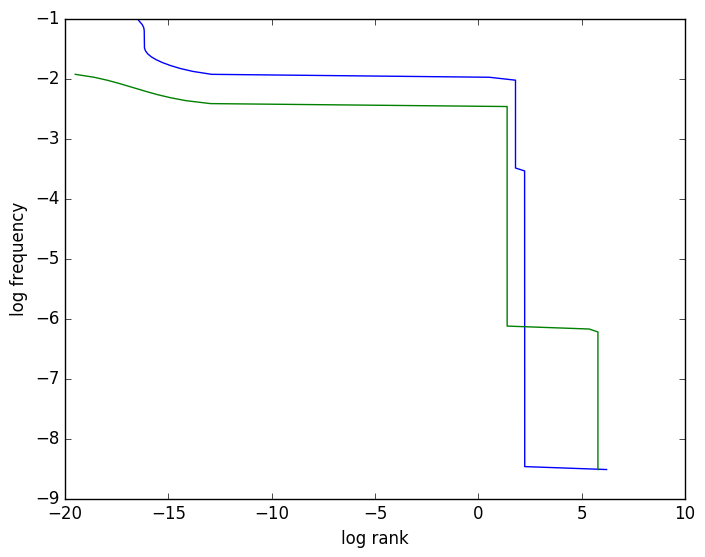
\includegraphics[width = 8cm]{exact_dists_plot}
	\caption{Frequency by rank of 2 corrections distribution. The distributions have steps containing many corrections that are just as probable with very low probability. 	\label{fig:corrections_dist}}
\end{figure}

\subsection{Assessment values} \label{subsec:Assessment-values}

In the previous section we presented empirical assessment of the distribution of
corrections to a sentence. We now turn to the consequent bias (under-estimation) in the estimation of a string-based similarity measure, for different values of $M$. Our goal is to assess what value of $M$ would be a sweet spot, which is both practical (as collecting references is costly) and reasonably biased.\lc{do we indeed assess the sweet spot? we only show the door someone must walk through it according to the budget he has}

We discuss two similarity measures. One is the sentence-level accuracy (also called ``Exact Match'') and the other is the GEC F-score.
 
\paragraph{Sentence-level Accuracy.}
Sentence-level accuracy is the number of sentences which were corrected in a way that exactly matches one of the
references (also called ``Exact Match''). While this score is less commonly used than F-score as an evaluation
measure of a corrector, it is a basic, interpretable measure and it is closely related to loss functions used for
training statistical GEC systems \cite{rozovskaya2010training,chodorow2012problems,rozovskaya2013joint}. 

Assume a set of test sentences $X=\{x_1,\ldots,x_N\}$,
and their gold standard references $Y_1,\ldots,Y_N$ . We define the
{\it coverage} of the references of the $i$-th sentence to be

\begin{equation}
  \footnotesize
  Cov\left((x_i,Y_i\right)=Pr_{y \sim \mathcal{D}_i}\left(y \in Y_i\right)
\end{equation}

Given a corrector $C$, we define $CP$ to be its probability to correct a sentence $\mathbb{E}_{x\sim{L}}Pr\left(C\left(x\right)\in Correct_i\right)$. We estimate $C$s quality by sampling a set of source sentences
$x_1,\ldots,x_N \sim \mathcal{L}$, and evaluate the quality of $C(x_1),\ldots,C(x_N)$ relative
to the source. 

Given a gold standard $Y$, we can compute the common accuracy score, which is an estimate to $CP$:

\begin{equation}
  \footnotesize
  Acc(C;X,Y) = \frac{1}{N} \sum_{i=1}^n \mathds{1}_{C(x_i) \in Y_i}
\end{equation}

With $Y_i=Correct_i$ this is an unbiased estimator. Unlike other fields, in GEC we showed collecting all $Correct_i$ as a reference is impossible. It is possible to get a good estimate of $Acc(C;X,Correct_i)$
by taking a large enough sample from $Correct_i$, which is the common practice in reference-based evaluation.
\begin{align}\label{eq:correction-in-gs}
  \footnotesize
  Pr[C(x_i) \in Y_i] = Pr[C(x_i) \in Correct_i] \cdot \\
  Pr[C(x_i) \in Y_i | C(x_i) \in Correct_i] = \nonumber \\
  CP\cdot Pr[C(x_i) \in Y_i | C(x_i) \in Correct_i]\nonumber
\end{align}

 However, since $Y_i \subset Correct_i$, the estimator will always underestimate $CP$.\lc{We gathered all the information for sampling without repetition too, are those interesting and should be discussed? They are useful if you gather in an unrepeated way and wonder how good is your coverage }
It's clear that the sample size $N$ does not affect $\mathbb{E}[Acc(C;X,Y)]$, but the number of references
might. Another property to consider is that under the reasonable assumption that $\mathbb{E}Pr[C(x_i) \in Y_i | C(x_i) \in Correct_i]$ is the same for $C$, $C'$ the ratio between their expected accuracy
is always the ratio between their $CP$s, no matter what the values of $p_1,\ldots,p_N$ are. Intuitively, if we assume the different systems corrections are independent from the way gold standard corrections were generated, than the ratio of accuracy scores reflects the ratio between their probability to have a valid correction.
So using $Acc$ score we get a reliable way of comparing $CP$ of two correctors,
but we underestimate $Acc\left(C;X,Correct_i\right)$ by the scale of $Pr\left[C\left(x_i\right) \in Y_i | C\left(x_i\right) \in Correct_i\right]$. The only way to decrease this bias
is to enlarge $p_i$, that is to say to enlarge $M$. 
We now proceed to estimating what sample sizes ($M$) give a good estimate of $CP$.\lc{make sure measure and score are being used consistently}

In order to gain insight into the accuracy measure, we need to know something about the distribution from which the given corrector chooses valid corrections. As each corrector might have its own biases, the most appealing choice would be to evaluate a corrector in which this distribution is the same as the one from which corrections for the gold standard are being drawn from. Formally, if $C\left(x_i\right) \in Correct_i$ then $C\left(x_i\right) \sim \mathcal{D}_i$. 

Thus, the second
term in Equation \ref{eq:correction-in-gs} is $p_i = \mathbb{E}_{Y_i}[Cov(x_i,Y_i)]$. Therefore $Acc(C;X,Y)$ is distributed as
a Poisson Binomial random variable (divided by $N$), with probabilities $\{p_i \cdot CP\}_{i=1}^N$. \footnote{A Poisson Binomial random variable is a sum of Bernoulli variables with different success probabilities.} We also assume our corrector is always correct (so $CP=1$), but as noted earlier any other value for $CP$ would only scale the results by $CP$.

 \begin{figure}
   	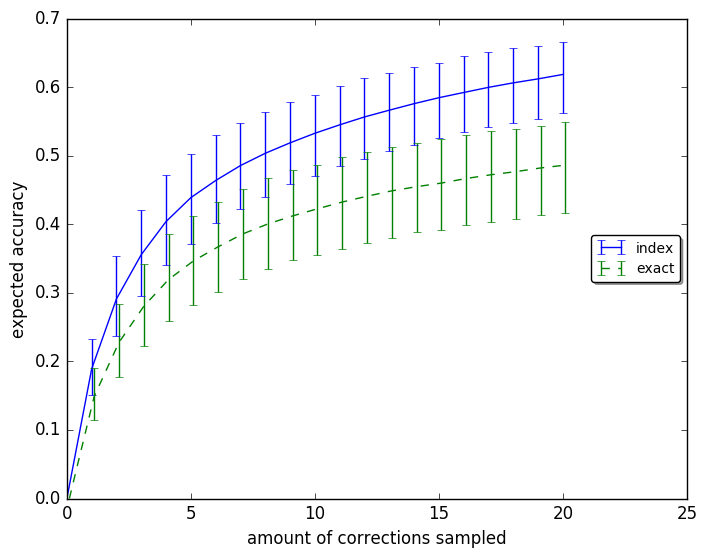
\includegraphics[width=8cm]{repeat_1000_accuracy}
 	\caption{Mean accuracy values for perfect correctors with different number of references.} \label{fig:accuracy_vals}
 \end{figure}

 Using the estimated $\mathcal{D}_i$ for each source sentence $x_i$, we can now compute $p_i$ for any
 size of $Y_i$ (value of $M$). However, as this computation is exponential in $M$, we estimate $p_i$ using
 sampling. Specifically, for every $M\in[20]$ and $i$ we sample $Y_i$ 1000 times, compute 
 the covered probability mass $Pr_{\mathcal{D}_i}[\{y: y \in Y_i\}]$ for each sample and estimate $p_i$ to be their
 average. The $p_i$ define the Poisson Binominal distribution of $Acc(C;X,Y)$.

 Figure \ref{fig:accuracy_vals} presents the expected values of $Acc(C;X,Y)$ according to our estimates of $p_i$ for
 different values of $M$. As our corrector is perfect, we would ideally expect its accuracy to be
 $Acc(C;X,Correct_i) = 1$. However, as the graph shows, even for values of $M$ which are much larger than
 those considered in the GEC literature (e.g., $M=20$), the expected accuracy is only of about 0.5.
 
 In order to examine whether our findings persist with a more relaxed measure, we examine the relaxed
 {\it Exact Index Match}, where two corrections $y$ and $y'$
 are equivalent relative to a source $x$ if in their alignments with $x$, $a$ and $a'$ respectively,
 if the number of deleted and added words is the same, and aligned words according to $a$ are
 changed (different from the aligned source word) if and only if, they are changed according to $a'$. Alignment is done in the same way as in \ref{sec:formal_conservatism}. Figure \ref{fig:accuracy_vals}
 shows that while expected accuracy is somewhat higher, still with $M=20$, it is no more than 0.65.
 
 To recap, we see that computing accuracy exactly requires many more references than was previously attempted.
 While common practice in GEC is to use $M=1$ or $M=2$, our simulations show that computing accuracy with
 so few references yields a scaling down of 5 or more. The graphs do show near linear behaviour from $M=9$ or
 so, which indicates that it reflects a reasonable balance between cost and bias.
 
 \paragraph{F-Score.}
 % present F-score
 % say that its analysis is more difficult
 % in order to estimate how different values of $M$ affect the bias of
 % the F-score, we use bootstrapping methods. again with a perfect corrector
 % explain briefly what we do.
 % show results
 % results are comparable to the index-based accuracy, i.e.,
 % an underestimation of the F-score
 % by a considerable factor for M=1,2, and they do not correspond to any natural point in the graph
 % near-linear behaviour with M=8, which is perhaps a practical solution
 While accuracy is popular as a loss function for training GEC systems,
 $F$-score is standard when reporting a corrector's performance.

 Computing F-score is not at all straightforward. The score is computed
 in terms of matches of {\it edits}, which are sub-strings of the source
 that are replaced in the correction, and in the reference. Since correctors
 do not normally produce edits, $F$-score is defined optimistically, maximizing
 over all possible ways to annotate the source with edits, so as to end
 up with the correction. 
 The resulting optimization problem is NP-hard, but designated scorers
 have been developed to estimate it, notably the $M^2$ scorer
 \cite{dahlmeier2012better}.

 Given the complexity of the definition of the measure, no analytical analysis is at hand (as with accuracy). Instead, we use a bootstrapping
 approach to estimate correctors' performance,
 incurred by the use of small values of $M$.
 % how do we measure?
 

% In GEC the $F$ score in use compares a set of system edits to a set of gold standard edits. As the task of GEC does not require edits from the correctors, complicated scorers  were created to estimate the closest edits and with it the $F$ score.

 % what do we measure? we evalaute a perfect corrector
 As with accuracy, we assume the evaluated corrector is perfect 
 (i.e., for every sentence $s$, it produces a correction in $Correct_s$),
 rather than the output of existing systems, both
 in order to avoid introducing any system-specific biases to the analysis,
 and the high cost of computing the true F-score of a system.

 % our results
 We assess different expected results for perfect outputs with different
 $M$ values (see \ref{fig:F_Ms}).
 It is a challenge to do that without generating a whole dataset with enough annotations plus a large test
 set to account for the variability of different annotators. We sample uniformly a sentence from the
 empirical data set for each sentence in the NUCLE test data that needed correction by the current gold standard.
 For each sentence we sample $M$ corrections as a gold standard and one correction to be the perfect corrector
 output. With that we use the many corrections for each sentence to account for annotation variability.
 At last, we transform each of the corrections into a set of edits as requested
 by the $M^2$ scorer.\oa{this needs to be much more formal. also discussion of difficulty should be at the end.}

 % discussion
 
In respect to the edits, we note that the score for $M=2$ is a bit lower than one would expect\oa{why should I expect this?}. This may result by the mechanical creation of edits. The different edits might give bias to the results\oa{but this is also true when evaluating real systems, no?}. Edit borders are not part of what correctors need to extract, in other words, it is an information that is not inherent to the task. Those edits are a disadvantage of the scoring system itself. It makes crowdsourcing much harder, and the edits are yet another thing that annotations often disagree upon(\cite{dahlmeier2012better}). It might be another reason that calls for use of another, more interpretable score.

This would be a good place to mention the drawbacks and assumptions of the methods we are using. We assume that the sentences we picked are a good representation of the overall sentences, but know they might be a bit simpler as we did not choose very large sentence for the reasons mentioned earlier. Another assumption is that the simple automatic edits are not making a big change in respect to the human edits.

To conclude, on both measures we see a large improvement in coverage when enlarging $M$ suggesting that a more reasonable $M$ to choose would be somewhere around 8 where the high probability corrections are probably covered and the graph turns semi-linear. The results also strongly support the hypothesis assessment values are very low, and hence might be a cause for over conservatism.
 Another conclusion to be made is that given a value from the assessment process we may estimate how low the value is in respect to the perfect assessment. Some may wish to correct for this under assessment.
 
\subsection{On significance and variation}

\oa{separate disucssion issues and put them in 3.6; this section is only
  technical, with some more explanation on bootstrapping}


So far we have discussed the mean values of the assessment and showed they are lower bounds of the true value, and for the small $M$ in use a substantially under-estimate of it. However, since measures are often used as means of comparison between different systems, not less important than the bias is the variance of these estimators, and subsequently the significance level we may obtain with them. 

\begin{figure}
   	\includegraphics[width=8cm]{$F_{0.5}$_Ms_significance}
	\caption{F Score results with different sizes of gold standard.\label{fig:F_Ms}}
\end{figure}
\begin{figure}
   	\includegraphics[width=8cm]{$F_{0.5}$_significance}
	\caption{F Score results for different correctors including confidence interval.\label{fig:F_correctors}}
\end{figure}


\paragraph{Accuracy:} As before, we start by considering the analytic formalism we have for accuracy. For that, sentences which were not corrected, or wrongly corrected have no variance with different $m$s, corrected sentences do. The variation of the Poisson binomial random variable we have is $\sum_{i=1}^{n}p_i\cdot\left(1-p_i\right)$ and as we divide the variable by $n$ we get $\frac{\sum_{i=1}^{n}p_i\cdot\left(1-p_i\right)}{n^2}$. 
The variation is proportional to the square of the number of sentences chosen given fixed $p_i$ values. Given a fixed $N$ variation gets lower as $p_i$s get away from $0.5$, a change that, from a certain point, occurs when $M$ is increased.

\paragraph{$F$-score:} Analyzing variance of $F$ score is intractable\cite{yeh2000more}, thus, we use bias-corrected and accelerated bootstrap \cite{efron1987better}, to assess the $95\%$ confidence interval of different correctors with the current NUCLE test data ($m=2$), based on the same process as in \ref{subsec:Assessment-values}. Results can be seen in \ref{fig:F_correctors}. The results supports our method of assessing as the bounds indeed cover the actual scores seen in all of the cases.

The results(\ref{fig:F_Ms}) suggest no great improvement of significance should be expected in the transition from $M=2$ to $M=5,8$. We can also learn from them what should be thought of as significant, for example the best performing corrector is significantly better than the second best we have checked, but is not significantly better than the other correctors proposed in the same article\cite{rozovskaya2016grammatical}.

\subsection{Discussion}
\com{migrated paragraphs:
	
	We wish to show a somewhat more complex point of view, stating that the way to reduce variation in assessment values would be to balance between the number of sentences and the number of annotations per sentence. We also provide the numbers needed for choosing how to balance wisely.\oa{so instead of computing variance, we compute the M,N balance} 
	
	Choosing how to balance is dependent on the goals of the one collecting data, and affects the mean value as well, as discussed in \ref{subsec:Assessment-values}. Thus, we will not discuss this issue here and just point out that such questions have been studied in various fields such as genetics\cite{ionita2010optimal}.
	
	So, why is significance more complicated? Basically, because variance is more complex than mean. While $\mathbb{E}_{y\sim d_x, x\sim L}\left(\hat{S}\right)$ vary only as we change $M$
	the number of annotations, but not $N$ the number of corrections,
	$Var_{y\sim d_x, x\sim L}(\hat{S})$ depends on both. We try to assess and give an upper
	bound on how much it varies for different $M$ and $N$, allowing
	for both a smart allocation of resources when building a corpus and for assessing on given corpora whether two correctors are actually different.
	}


\oa{discuss RoRo higher than perfect scorer; explain why perfect is not necessarily
  maximizer of F-score (even with knowledge of all possible corrections);
  say that RoRo doesn't make enough changes, so it's far from perfect (according
  to the gold standard), but still it obtains comparable (and even higher
  performance) than a perfect corrector, which is severely penalized for selecting
  random valid corrections, which are likely not to be in the gold standard
  due to the small value of $M$.
  at the end explain what other factors may contribute to this difference}

\oa{say that large N values are sufficient for comparing systems (significance),
  but it will not solve the other problems: under-estimation of true performance,
  over-conservatism, possible issues when training systems etc.}

If the NLP community has agreed one correction is not enough\cite{tetreault2008native}
we can now say 2 is no magic number either. The gain from each annotation in respect to mean value is still high and only at about 8 becomes semi-linear. We can also see the effect of different references amounts on significance and mean value of both accuracy and precision, recall and F score.
We see that considering the changed indexes, looking for example at different synonyms as the same correction, still holds a very large number of different corrections for every sentence.

Perhaps less obvious will be how low coverage affects the development
process. Even if corrected well, sentences which have more possible
corrections will grant lower scores on precision for correcting, while recall will not grant high reward for correcting, as most of the time the correction will be considered false anyway. This, and especially in the precision oriented scenario, will lead implicitly in algorithm development cycles, to learn \textbf{not} to correct those sentences at all. Also, consider any machine learning algorithm which somehow represents the notion that not correcting is more important than false correction. An example for such algorithm would be one that uses a loss function with a special case for the output equals the input. Such algorithms would also learn to avoid correcting, as corrections would most likely result in high loss, even when their correction is actually valid.
In the rest of this section we will show that the assumptions we made are the current reality. 


\section{Semantic Similarity Measure}\label{sec:Semantics}

%Conservatism is considered an important trait for a corrector, reflected for example
%in the selection of $F_{0.5}$, which emphasizes precision over recall, as the
%standard evaluation measure in GEC.
%In the previous section we followed the common approach in GEC evaluation and evaluated

%The thought that stands behind such emphasis is that a user
%would be understanding towards errors he did, of which he is probably
%not even aware, not being corrected, but would not be so understanding
%of corrections altering what he meant to say, in a way he perceives as wrong.

In this section we explore an alternative approach to overcoming over-conservatism
incurred by reference-based similarity measures in the presence of a large set of
valid corrections, the semantic similarity approach.
Semantic similarity is established not by computing the string similarity between
the reference and the correction, but by computing the similarity in their semantic
structures. As semantic structures represent an abstraction over different realizations
of a similar meaning, we anticipate that such measures would result in a similar
effect as to taking a large value of $M$ without enumerating all possible corrections,
which may be prohibitively difficult.

Concretely, the measure is defined as a graph distance measure between
semantic graph representations that reflect the meaning of the source
sentence and the correction.
We note that such a measure needs to be complemented with an additional
measure of fluency or grammaticality, as it only captures
the faithfulness dimension, namely the extent to which
the meaning of the source is preserved in the correction,
and not the grammaticality of the correction.\oa{we could cite the fluency people from ACL? or maybe fluency scores from MT evaluation?}

Concretely,
we use the UCCA scheme as a semantic representation \cite{abend2013universal}, motivated by
its recent use in semantic machine translation evaluation \cite{birch2016hume},
and present results from two experiments that support the feasibility of the approach.
First, we show that a semantic annotation can be consistently applied to LL,
through inter-annotator agreement experiments.
Second, we show that a perfect corrector scores high on this measure, unlike with
the multi-reference measures disucssed in Section \ref{sec:increase-reference}.

%as LL consists of many grammatical mistakes that makes syntactic
%analysis ill-defined for the task. We show evidence that this is the case, by having
%two annotators annotate a sub-corpus from the NUCLE dataset, and by measuring their
%inter-annotator agreement.
%%%Second, we ask whether corrections for a sentence indeed need to be faithful to the source. We seek to answer this question by measuring
%the semantic similarity between the source and the reference. We show support for an affirmative answer to this question 
%by annotating the references provided for the NUCLE dataset,
%and detecting high semantic similarity between the corresponding sentences on both sides. 

%\subsection{Background}

%Reliable assessment by a gold standard might be hard to obtain (see
%\ref{sec:increase-reference}), and human annotation for each output
%is great \cite{madnani2011they} but costly, especially considering the 
%development process. Under these conditions,
%%given a reliable semantic annotation we can enhance the reliability of our assessment. A simple way to do it is to somehow account in the assessment score for semantic changes. 
%Another, more ambitious way to do that might be to decouple the meaning
%from the structure. We propose a broad idea for a reduction from grammatical
%error detection and a comparable semantics annotation to grammatical
%error correction assessment. Lets assume we have both a reliable error
%detection tool and a good way to measure semantic changes. Then, we
%can transform assessment to a 3 steps assessment. 
%Step one, detect errors in the original text. Assess the amount of needed corrections, and the percentage of which that were changed.
%Step two, assess how much did the semantics change.
% Give a negative score for changing semantics.
%Last step, use
%the error detection again to assess how many errors exist in the correction
%output, whether uncorrected by the corrector or new errors presented
%by the correction process itself. 

%This assessment was partially inspired by the WAS evaluation scheme \cite{chodorow2012problems},
%in short it states we should account in the assessment for 5 types,
%not only the True\textbackslash{}False Positive\textbackslash{}Negative
%but also for the case where the annotation calls for a correction,
%and the corrector did a correction, but one that is unlike the annotation's
%one. With the proposed assessment we can measure how many of the corrections
%were corrected correctly (First + Second), and how many errors do
%we have eventually (Third) and combine them to get something similar
%to the Precision Recall that is widely used. We can also account for
%the places where the error was detected and check if it was corrected
%in a way that makes it grammatical and did not change semantics, the
%fifth type. We do that without getting a human to confirm this is
%indeed a correction.

%This system would be even more informative than the current one. Allowing assessment of
%what subtask exactly did the corrector fail to perform. Answering questions
%like: was the corrector too conservative and did not make enough corrections?
%Was it making changes in the right places but not correcting grammar successfully?
% as the corrector correcting grammar but changing things
%it was not supposed to? etc.

%Semantic structures were used for LL tasks \cite{king2013shallow}, but so far not to GEC. Some syntactic representations were suggested for this task, and as they are popular for structural representation we devote the next subsection to discuss them. Specifically we explain, why, apart from not being based on semantics, syntactic representation is not a good fit for LL and in particular not for enhancing the evaluation without enlarging reference number.

\subsection{Structural Representation in LL}

The usefulness of syntactic parsing in NLP has encouraged a number of previous
projects to define syntactic annotation in the context of LL.
%Most work on structural representation in LL has focused on syntactic (rather
%semantic structure).
Defining syntactic structure in this context is difficult, as the syntax employed
by a language learner may not conform to any known syntactic framework.
While linguistic theories propose that each learner
makes a consistent use of syntax (even if this use does not conform the 
syntax of the learned language) \cite{huebner1985system,tarone1983variability},
this proposal has not, to the best of our knowledge, been adapted into a workable
annotation scheme.

Existing approaches to syntactic representation of LL in NLP
differ as to how to annotate erroneous use of syntax.
\newcite{berzak2016universal} and \newcite{ragheb2012defining}
annotate syntactic structures according to the syntax actually used
by the learner, regardless of the grammaticality of the use of this
syntax in this context.
The difficulty with this approach is that it may be unreliable as
a source of semantic information about the sentence, as semantically similar
sentences, formulated by different learners, may have considerably different
structures. \newcite{nagataphrase} takes an opposite approach, and attempts
to be faithful to the syntax intended by the learner. However, their
approach faces difficulties due to the multitude of different syntactic
structures that can be used to express a similar meaning.

%Syntactic representation is very popular and useful in many NLP tasks 
%\cite{mesfar2007named,ng2002improving,zollmann2006syntax}.
%Thus, one thought that comes to mind is to use grammar annotation 
%for LL.
%While not useless, grammatical approach is not well
%defined, and unclear both practically and theoretically.

In this section, we propose using semantic annotation as a structural
representation of LL text. Semantic structures are faithful to the intended
meaning of the sentence, and not its formal realization, and thus face
less conflicts where the syntactic structure used diverges from
the one intended.\oa{are there any semantic schemes you can mention in this context? we need
a connecting sentence/paragraph to connect it to the explanation about UCCA.}


\paragraph{UCCA.}\label{sec:ucca}

UCCA is a cross-linguistically applicable semantic annotation scheme. Formally, 
a UCCA annotation for a sentence $s$ is a labeled directed acyclic graph $G$, whose
leaves are the words of $s$. For every node in $G$,
we define its yield to be its leaf descendants. The
semantic units for $s$ according to $G$ are the yields
of nodes in $G$.

In the DAG edges are labeled with the relation the child has to the broader semantic unit
the parent represents. UCCA's basic unit is a \textit{Scene} describing an action or a state
that persists in time. In a \textit{Scene} there may be other \textit{Scenes} or scene elements
such as \textit{Participants}, \textit{Adverbials} or \textit{Time}.

Importantly, UCCA's categories, being semantic in nature, directly reflect the intended
meaning of the sentence, and not its form. Indeed, \newcite{sulem2015conceptual} has found
that UCCA structures are preserved remarkably well across translations.
Therefore, UCCA can be applied to grammatically erroneous
sentences which nonetheless have a coherent meaning, without requiring any adaptations
to the annotation guidelines, or the use of auxilliary annotation.


\subsection{Experimental Setup}

We employed two annotators, fluent in English and with background in translation.
Their training included jointly annotating both LL and standard English
passages, until a high enough agreement was reached (6 hours of training in total).
Training passages were excluded from the evaluation.

We experiment on 7 essays and their corrections from NUCLE, each of about 400 tokens.
In order to measure inter-anntoator agreement, we assigned 4 essays to both annotators
and compute their agreement (Section \ref{sec:iaa}).

In order to measure the score
of a perfect corrector, relative to the source, we compute a similarity measure
between the UCCA annotations of the NUCLE LL essay and correction.

For the different experiments 20 paragraphs were annotated, a table with the full
information can be found in the appendix \ref{tab:annotated-paragraphs}.Overall, 2 LL
and 2 corrected paragraphs were annotated by both annotators, 9 parallel paragraphs were
annotated by the same annotator and 6 by different annotators.

\subsection{Inter-Annotator Agreement}\label{sec:iaa}

We compute inter-annotator agreement over 4 LL essays, 
To measure the similarity of two annotations $G_1$ and $G_2$ over the same set of leaves,
we use a generalization of the parsing F-score metric to DAGs, where an
edge $(v_1,u_1) \in G_1$ is said to match an edge in $(v_2,u_2) \in G_2$ if
they have the same label, and if the leaves
reachable from $u_1$ are the same as those reachable from $u_2$. 
(this measure collapses to the common parsing F-score if $G_1$ and $G_2$ are trees)

We obtained an F1 score of 0.845 (Precision 0.834, Recall 0.857), which
is comparable to the IAA reported for English Wikipedia texts by \cite{abend2013universal}.
As another point of comparison, we computed IAA over a corrected paragraph in NUCLE,
obtaining a similar F-score of IAA.

These results suggest that annotating LL with UCCA does not lead to any degradation
of IAA, and can be applied as consistently to LL text as to non-LL texts.

%We see that as enough to be a proof that UCCA can be applied to LL, especially considering those numbers
%are a bit higher than the IAA originally reported
%for native English .
%We explain the rise in agreement by the fact that the guidelines and
%procedures were refined since UCCA was first introduced and not to
%superiority of UCCA for annotating LL. A similar F1
%score for IAA (0.849) over corrected paragraphs
%suggests the same.

%At least theoretically, semantics are well defined even on ungrammatical
%text. With the right tools we might capture at least some of the semantics
%of sentences and use them for the same purposes of grammatical annotation.
%In this work we will use Universal Conceptual Cognitive
%Annotation (UCCA)\cite{abend2013universal}, we will show that practically
%there are semantic annotation schemes that can be used for the purposes discussed.


\subsection{Semantic Faithfulness Score}

%After showing we can rely on the UCCA annotation for LL, the next experiment
%aims to check our hypothesis that indeed when correcting we expect faithfulness.




We now turn to defining a semantic measure of faithfulness. 
To do so, we compare the UCCA annotation of the source sentence and its correction. 
As there are no existing methods for comparing UCCA annotation 
We propose several new methods to compare UCCA annotation of a LL with UCCA annotation of corrected texts.

Giving a more accurate
measure than the upper bound suggested by \cite{sulem2015conceptual} for
comparing two parallel texts in different languages, while keeping
the essence of comparing how many of the aligned nodes conserve meaning and tag. For that we may think for a moment on GEC as
translation from LL to Proper English, and a good translation
would be a translation which keeps the meaning but has the syntax
of English. Considering that, just like in translation, we can align words from the LL to the corresponding words in English
and keep record of how many of those nodes kept their labels.

As comparing labels is trivial, and done before us. We should focus on how we propose to align nodes. 
First, note that comparison should not be at
the token level, as we want to allow tokens to be corrected - replaced or removed -
as long as the higher structures convey the same meaning. We thus
prune the labels above the leaves, the tokens of the sentence. To
define an alignment of the nodes, we suggest some possible ways, all
based on first aligning the words in order to give order to the DAG and then comparing the structure in one way or another.

We align words in the same manner explained in \ref{sec:formal_conservatism}.
As to aligning nodes, we can use word spans of each node, based on
the token alignment and the DAG structure, to choose how best to align.
A first and most straightforward approach would be to compare all
pairs of nodes in parallel paragraphs and to each node from one paragraph
assign the one most similar node, span wise from the other. That approach
is quite similar to the IAA aligning, but it
has three drawbacks; it is asymmetric; it may be over optimistic aligning
nodes without considering the DAG structure; and it might be
slow for many nodes. Being asymmetric is not much of a problem. If we thrive for symmetry
we can compute the measure twice and use the results mean,
that would also be the case for other asymmetric methods we suggest.
In order to address the other drawbacks we propose different aligning methods.

A second method driven by the assumption that nodes higher in the
hierarchy are more important to the semantic representation is measuring
the largest cut in which nodes are aligned (top down) to each other
and have the same labels. This is a harsher lower similarity
score but one of which might be more representative of the semantics
that are kept and hopefully more informative for tasks that will use it.

A third type of methods were token similarity methods, these methods
use one kind of aligning (top down, bottom up or pairwise) and only
compare the meaningful nodes. This was called upon by \cite{sulem2015conceptual}. 
This approach makes sense due to the fact that some labels
are well defined and thought upon while others are still vague and
call for future work on refining or adjusting them, moreover, some
labels are more semantic while other labels are currently just a place
holder as each node must get a level, and the semantic role is not
always clearly defined (e.g. the word ``is'' in ``he is walking''
seem to be more syntactically related than semantically. In UCCA it is tagged as a \textit{function} word.). The unused
labels are center, elaborator, function, relation, linker, ground
and connector.

A bit different way than all the others is to compute the labeled
tree edit distance\cite{zhang1989simple}, for that we first needed
the trees to be ordered, we did that in a top down fashion. An interesting
future work would be to use unordered tree edit distance methods\cite{zhang1992editing}.









In order to control for differences between the annotators, we explore both
a setting where the two annotations were annotated by the same annotator,
and settings where they were annotated by different annotators.


\oa{the following paragraph should be a footnote}
While planning the experimental setup a small obstacle occurred,
there exists no measure for how similar two different UCCA annotations of different texts are.
We considered using suggested semantic measures
such as SMATCH\cite{cai2013smatch} but it can not work for UCCA or
DAG similarity measures such as graph kernels (e.g.\cite{kashima2003marginalized}),
but those tend to work on bigger graphs and would be the wrong tool
for the small UCCA DAGs. Thus, a new measure is called upon.

%%

\lc{Where should that appear? in footnote?}All of the code used for this paper is given as a \href{link will be disclosed upon publication}{contribution}.
\vspace*{-\baselineskip}
\begin{table}[h!]
	\centering
	\singlespacing
	\begin{tabular}{c|c|c|c|c}
		Annotator & Edit & Fully aligned & Top down & Token analysis
		\\
		\hline
		Same & 323.16 & 0.78 & 0.79 & 0.85
		\\
		Different & 209.55 & 0.85 & 0.87 & 0.89
		\\
		\end{tabular}
		\caption{Different UCCA distance measures between LL and corrected parallel paragraphs. The scores are quite similar to the IAA, which means distances are indeed low.\label{tab:Distances}}
	\end{table}
\vspace*{-\baselineskip}
	\subsection{Results}
	
	We present in \ref{tab:Distances} the scores of the different presented
	methods. For each method we present the average results of pairs
	of paragraphs annotated by the same annotator and pairs where each
	paragraph was annotated by a different annotator.
	
	Finally, we present as a control measure and a bound on the best score
	we can expect to get in such comparison the scores of paragraphs
	in which we compare two annotations for the same paragraph using all
	the similarity measures discussed, it can be thought of as a different
	way to defining IAA. Note that a similarity
	of 1 and distance of 0 is indeed reached when comparing an annotation with itself.
	
	In \ref{tab:Token_analysis} we present the results of the token analysis, the
	upper bound suggested by \cite{sulem2015conceptual}, showing similar
	results for LL - corrected tuples as those seen in English
	- French comparison.
\vspace*{-\baselineskip}
		\begin{table}[h!]
			\centering
			\begin{tabular}{c|c|c}
				Annotator& As+Ds & Scenes\\
				\hline
				Same  & 0.97 & 0.96\\
				Different & 0.96
				 & 0.93
				 \\
				\end{tabular}
				\caption{Token analysis F score for similarity in UCCA labels between structures in LL and corrected parallel paragraphs. The similarity is evidently very high.\label{tab:Token_analysis}}
				\end{table}
				
	\subsection{Discussion}
	In our experiments we show that a perfect corrector receives a high faithfulness score using the suggested measures. Unlike the former measure it requires annotation for the source and no references at all, solving a lot of the problem of references.
	
	The experiments show the measure is usually not sensitive to differences between the LL essays their corrections. The other direction is important as well: what the measure is sensitive to. This, of course, depends on the scope of distinctions covered by the semantic annotation. In UCCA's case, it is argument structure, the connections between scenes etc. We attempted to empirically show that the measure
	captures semantic unfaithfulness by the corrections proposed by existing systems, but cases of structural (rather than lexical) corrections are rare, which prohibited such an experiment.\footnote{In fact, this how we arrived to the findings in section \ref{fig:over-conservatism}} We expect that once correctors are less conservative, this evaluation will be made possible.
	
	
		\lc{from here to the end needs revising}
	From the result we learn a number of things, the upper
	bounds in table \ref{tab:Token_analysis} suggest high stability of UCCA over GEC, and the results are similar to those shown over
	translation. This upper bound seem not to be very strict if the other
	measures are to be considered true values. 
	However, due to aligning errors those measures are actually a close lower bound more than they are an exact value.
	
	We see that measurements for symmetry that are similar to the inter
	annotator agreement measure also suggest high stability, achieving
	scores not much lower than the one different annotators get for the
	same paragraph. This result is quite strong as an inter annotator
	agreement is the upper bound being the score of comparing a paragraph to itself. 
	Most importantly we learn from it all that even when correcting grammatical errors, the semantic structure (as represented by UCCA at least) is hardly changed and thus can be used as a tool to avoid introducing semantic changes when trying to only change grammar. 
	The symmetry measures we introduce can be used to enforce semantic conservatism.
	In conclusion, we have shown some direct ways to measure
	semantic faithfulness. Such ways will allow correctors to be less formally conservative while controlling semantic conservatism. Thus, focusing on what users - and hence we - are more interested in.

\subsection{Faithfulness and conservatism - not only due to reference number}
	In many of the uses for correction,
		the user does know his grammar is not perfect and would accept
		a change in grammar when needed. Because of this approval we also
		hypothesis, and it may call for a user study to prove or disprove
		this hypothesis, that users might accept a correct text unit of theirs
		being corrected to another correct text unit with the same meaning.
		This would be an example of being faithful but not conservative.
		Maybe even more importantly, we aim to have as many correct sentences
		as possible, but as neither the grammar is fully correct in the first place,
		nor is the user's understanding of it, failing to correct grammar
		is acceptable. Changing meaning will be totally unacceptable, and
		also surely detectable by the user. In other words, the users do expect
		the corrector to be active and not too conservative, but
		only as long as it is faithful. 
		
		Moreover, as correctors are based on statistics, they might even
		just correct to a more common way of saying the same thing. Such unnecessary
		correction is not conservative, and at GEC maybe be unwanted, but not strictly unwanted as overall
		it is still faithful. Additionally, some may even
		consider such correction a needed one because it has a better grammar considering
		Fuzzy Grammar\cite{lakoff1973fuzzy,madnani2011they} or a more fluent
		way to say the exact same thing. The latter was recently suggested as a necessary
		shift in the goals of GEC\cite{sakaguchi2016reassessing}.
		Considering all this, we propose that next generation correctors and evaluation will be focused on faithfulness
		when possible rather than on conservatism. Of course that with the evaluation comes the development and it all suggests that it might be beneficial to incorporate faithfulness not only for assessment but also as a feature for correctors. 

\bibliographystyle{acl2012}
\bibliography{propose}

\appendix
\section{Annotated paragraphs}
\begin{table}[]
	\centering
	\begin{tabular}{lll}
		Annotator-id & NUCLE-id & type      \\
		1         & 2  & corrected \\
		2         & 2  & corrected \\
		1         & 2  & learner   \\
		2         & 2  & learner   \\
		1         & 3  & corrected \\
		2         & 3  & corrected \\
		1         & 3  & learner   \\
		2         & 3  & learner   \\
		1         & 5  & corrected \\
		2         & 5  & corrected \\
		1         & 5  & learner   \\
		2         & 5  & learner   \\
		1         & 6  & learner   \\
		2         & 6  & learner   \\
		2         & 7  & corrected \\
		2         & 7  & learner   \\
		1         & 8  & corrected \\
		1         & 8  & learner   \\
		1         & 10 & corrected \\
		1         & 10 & learner  
	\end{tabular}
	\caption{The list of paragraphs annotated, showing which annotator annotated it, which type of language is used in it and the corresponding id in the NUCLE corpus. Note that parallel paragraphs have the same id.\label{tab:annotated-paragraphs}}
\end{table}
\end{document}
